\chapter{Problem Space Analysis}
\thispagestyle{plain}

\label{ch:psa}

\begin{figure}
\centering
\includegraphics[scale=0.70]{pics/ladybug-cities-solutions.eps}
\caption{Problem-Solution Map for a 5-city TSP.  Hollow circles represent the locations of the four static city locations, and the axes represent the $x$ and $y$ coordinates of possible locations of the fifth city.  The map shows eight unique high-quality solutions for all possible problem instances at the given granularity.  (Best viewed in color.)}
\label{fig:ps-map-ladybug-marked-cities}
\end{figure}

\begin{figure}
\centering
\includegraphics[scale=0.16]{pics/knapsack-400-ideal-with-labels.eps}
\caption{Problem-Solution Map for knapsack problem.  Axes represent the possible weight and value characteristics of one additional item that the planner may add to the knapsack.  The map shows 11 unique high-quality solutions for all possible problem instances, for objects in the integral weight and value range [1,100].  (Best viewed in color.)}
\label{fig:ps-map-knapsack}
\end{figure}


I use the term \textit{problem space analyais} (PSA) to describe methods that attempt to estimate the solutions for a large number of problem instances by analyzing patterns of solutions of a small number of problem instances.  In many domains, problem instances that are adjacent when indexed by their \textit{variable features} tend to have the same or similar solutions.  This chapter describes seven PSA algorithms for plan adaptation and presents a complexity analysis in the final section.



A graphical rendering of a Problem Solution (PS) Map for a set of small Traveling Salesman Problems (TSPs) is shown in Figure \ref{fig:ps-map-ladybug-marked-cities}.  The static characteristics are the x- and y-coordinates of four destinations that are common to all the problem instances (i.e., that the initial plan solution uses), plus the location of the start of the path (at the central solid circle).  The coordinates of the destinations are (10,10), (20,30), (5,35), and (35,25). The variable features of the problem instances are the $x$ and $y$ coordinates of a fifth destination, that could be added to the route as a dynamic change that requires plan adaptation.  The ranges of these latter features -- the $x$ and $y$ coordinates of the added fifth destination -- are represented by the  axes of the PS Map.  At each location in the map, the shortest route for the new five-city problem is generated as the solution.  Finally, each unique solution, consisting of a sequence of city identifiers, is assigned a color and plotted.  For example, (20,10) represents a problem instance in which the fifth city is located at (20,10), and has a shortest path solution of 0-5-1-3-2-4.  Proceeding in this fashion results in a mapping between each DTSP problem instance and the solution representing the shortest route.

As another example, a PS Map for a set of 0-1 Knapsack Problems is depicted in Figure \ref{fig:ps-map-knapsack}.  The knapsack problem requires the solver to select from a set of available items, each with a value and a weight, such that the total value of items selected is maximized and the total weight is below a threshold.  Intuitively, one wants the contents of knapsack to be as valuable as possible while not being too heavy to carry.  The 0-1 variant specifies that a maximum of one instance of each item may be selected.  This PS Map represents the problem domain in which a solver has already selected from a set of items and encounters a new item to consider adding to the knapsack, potentially displacing a current item.  Each problem instance's static characteristics is a set of 22 items, each with a weight and value; this is analogous to the TSP's fixed city locations.  The problem instances have two variable features, consisting of the weight and value of the new item, which are used as the axes of the PS Map; this is analogous the $x$ and $y$ coordinates of the additional destination in the TSP.  The solution at any point in the map is the set of items chosen by the solver where the pool of available items consists of the 22 static items plus the new item that has weight and value as represented by the coordinate location within the PS Map.

The dimensions of the PS Maps are represented as ordinal domains, which requires the ability to enumerate the values of each dimension.  Planning problems containing dimensions with discrete domains must define an ordering of the values and nearness metric that defines how ``close'' any two values are.  For example, a ``color'' dimension with domain \{red, green, blue\} must define a strict ordering and nearness metric in order to be used by the algorithms described here.  Dimensions consisting of real values must define a granularity to be used within the algorithms.

There is also an implicit assumption that similar problem instances have similar solutions when indexed by the problem characteristics.  If this assumption holds, then problem instances with similar solutions will appear in homogeneous groups within the PS Map, which is the feature that these algorithms exploit. In the case that a domain does not adhere to this assumption, there are methods, analogous to the SVM kernel trick, that may allow for my algorithms to be applied.  These ideas are discussed in Chapter \ref{ch:future}  as future work.


As previously mentioned, it is impractical to generate a high-quality PS Map through brute-force mechanisms.  For example, finding a high-quality map for a problem space with four fixed and one variable city, consisting of 12,000 problem instances, can be generated in less than a second with my current implementation on a circa-2015 standard laptop.\footnote{ASUS laptop with an Intel i5 1.70GHz CPU processor, running a single-threaded Java process with a 2GB memory limit.}  However, the PS Map for the same problem with two variable cities requires solving $\textrm{12,000}^{\textrm{2}}$ problem instances, which would take approximately three hours to complete.    Adding more dimensions of variability increases the size of the PS Map exponentially.\footnote{Note that, while increasing the variable city locations increases the number of TSP instances to be solved, each individual problem instance remains a static TSP.}  Since real-world problems can have many more dimensions and problem instances than in these experiments, it is imperative to develop efficient approaches for creating approximate PS Maps.

%\footnote{In order to generate the PS Map in a timely manner, the location of the second city was restricted to a subregion of the space, limiting the space to 311,000 instances which required 20 minutes to generate.}


I present seven novel techniques for creating PS Map approximations.  These techniques were conceived in somewhat linear fashion, such that subsequent algorithms take advantage of insights gleaned from the results of prior algorithms.  All seven methods begin with generating high-quality solutions to a random sample of problem instances, computed using heuristic search.  The \textit{sampling-classification} (SC) and \textit{sampling-classification with bias} (SC+bias) techniques use the solved problems and their  solutions as a training set to classify new problem instances into one of the solutions discovered during the initial sampling.  The former uses random selection to select the initial problem instances for solving.  This is the simplest algorithm and was the first attempt to validate the plausibility of the overall approach to PS Map approximation, and thus could be viewed as a baseline for subsequent approximation algorithms.  The latter attempts to bias the initial random selection towards problem instances that are close to the borders between solution regions. The \textit{solution border estimation} (SBE) technique uses the heuristic search objective function and the solutions of the sampled instances to estimate where the boundaries between solution clusters lie.  The \textit{select from sampled solutions} (SSS) technique applies each known solution to an unsolved problem instance and assigns the solution with the best utility.  The \textit{sampling-classification with active learning} (SC+AL) technique attempts to bias computational time towards solving problem instances  that are potentially ambiguous.  The \textit{support vector machine} (SVM) technique utilizes a support vector machine (SVM) to classify problem instances into solutions.  The \textit{support vector machine with solution border estimation} (SVM+SBE) technique also utilizes an SVM, but augments the training samples by finding problem instances near the borders of solution regions.  These methods are described in more detail below.  This chapter then concludes with a complexity analysis of the algorithms.

%\begin{comment}
%\scriptsize


%\begin{table}
%\begin{center}
%  \begin{tabular}{|p{1cm}|p{1.5cm}|p{1.4cm}|p{2cm}|}
%    \hline
%    & \textbf{Initial Sample} & \textbf{Solution Assignment} & \textbf{Domain Assumptions}\\ \hline
%    \textbf{SC} & Random & Polling of nearest neighbors & Similar problems have similar solutions\\ \hline
%    \textbf{SC+bias} & Near-city bias & Polling of nearest neighbors & Cities indicate solution borders\\ \hline
%    \textbf{SBE} & Random & Calculates solution borders & Solver objective function is continuous\\ \hline
%    \textbf{SSS} & Random & Selects best of known solutions & Solutions are repetitive\\
%    \hline
%  \end{tabular}
%  \caption{Summary of PS Map approximation approaches}
%  \label{tab:summary-of-approaches}
%\end{center}
%\end{table}

%\normalsize
%\end{comment}


\begin{algorithm}
\caption{Sampling-Classification}   
\label{alg:sc}
\small
\begin{algorithmic}[1] 
  
  \State Let $alpha \in (0.0,1.0)$
  \State Let $sampleRate \in (0.0,1.0)$
  \State Let $problemSpace \leftarrow$ set of problem instances
  \State Let $pollingRadius \in \mathbb{Z}^+$ 
  \State $totalNumSamples \leftarrow |problemSpace| * sampleRate$
  \For{$1 \dots totalNumSamples$}
    \State Randomly select unsolved problem instance
    \State Generate solution for unsolved problem instance
    \State Add problem instance \& solution to PS Map
  \EndFor

  \ForAll{$u \in$ unsolved problem instances}
    \State Let $rad \leftarrow pollingRadius$
    \While{$u$ is unsolved \& $rad < \textit{radiusOf}(problemSpace)$}
      \State Score solutions of problem instances within $rad$ of $u$
      \If{there is a solution with a unique maximum score}
        \State Assign solution to $u$
      \Else 
        \State $rad \leftarrow rad * 2$
      \EndIf
    \EndWhile
    \If{there does not exist a unique solution with the maximum score}
      \State Randomly choose one of the top solutions
    \EndIf
    \State Add problem instance \& solution to set of pending entries 
  \EndFor
  \State Add pending entries to PS Map 
\end{algorithmic}
\end{algorithm}


\section{Sampling-Classification (SC)}
The \textit{sampling-classification} (SC) technique (Algorithm \ref{alg:sc}) computes solutions to a random sample of the problem instances, then uses an expanding fixed-radius neighbor classification to assign solutions to the remaining (unsolved) problem instances.  Figure \ref{fig:sc-steps} illustrates the steps involved.  First, an initial random sample of solutions is solved by the heuristic solver (a).  Next, solutions to unsolved problem instances are assigned by polling the solutions of the sampled problem instances within a specified radius (b).  Finally, if the polling does not result in a plurality, then the polling radius is doubled until a plurality is achieved (c).  Polling does not include inferred solutions; each unsolved instance is assigned a solution based solely on the solutions to the original sample of problem instances.  Thus, the order in which the instances are solved does not affect the configuration of the resulting PS Map.

A visual example of the effect of this algorithm is demonstrated in Figure \ref{fig:initial-sample-tsp-addl}, which depicts an initial sampling of an problem space, and Figure \ref{fig:sc-approx-ps-map-addl}, which depicts the resulting PS Map after running the SC algorithm.

\begin{figure}
\begin{center}
    \includegraphics[scale=1.0]{pics/sc-steps.eps}
    \caption{SC procedure.  The dot represents the problem instance for which a solution will be inferred, and the solutions to sampled problem instances are represented by letters.}
    \label{fig:sc-steps}
\end{center}
\end{figure}

\begin{figure}
\begin{center}
    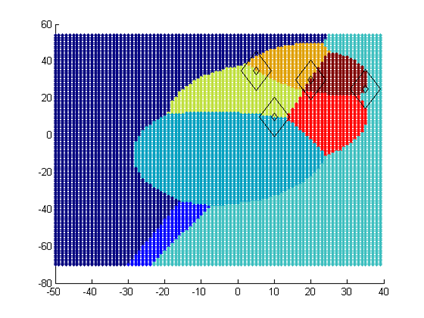
\includegraphics[scale=1.0]{pics/addl/ideal-ps-map.eps}
    \caption{Ideal PS Map of a five-city TSP}
    \label{fig:ideal-ps-map-addl}
\end{center}
\end{figure}

\begin{figure}
\begin{center}
    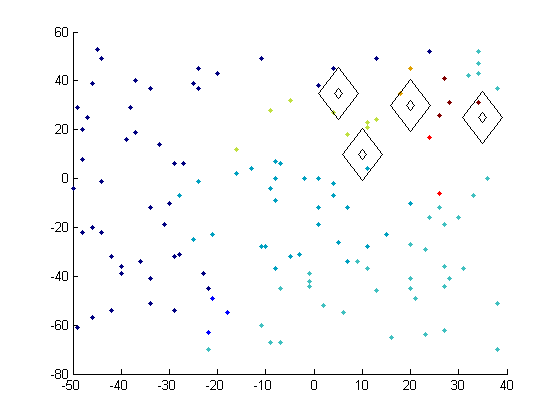
\includegraphics[scale=1.0]{pics/addl/initial-sample-tsp.eps}
    \caption{Possible initial sampling of a TSP problem space.  Points represent individual problem instances color coded by their solution.}
    \label{fig:initial-sample-tsp-addl}
\end{center}
\end{figure}

\begin{figure}
\begin{center}
    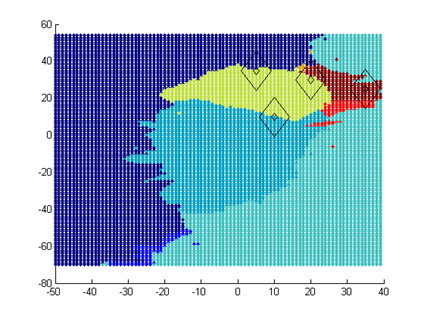
\includegraphics[scale=1.0]{pics/addl/sc-approx-ps-map.eps}
    \caption{Approximated PS Map generated by applying the SC algorithm to the initial sampling in Figure \ref{fig:initial-sample-tsp-addl}}
    \label{fig:sc-approx-ps-map-addl}
\end{center}
\end{figure}

\begin{figure}
\fbox{\begin{minipage}{1.0\textwidth}
Let $F = \{f_1, f_2, \dots, f_n\}$ be a set of fixed points, $o$ be the start of the tour, and $p$ be a variable point.  An optimal solution to the TSP problem is a sequence $S = \{s_1, \dots, s_{n+2}\}$ of the points $F \cup \{p,o\}$ such that $\sum_{i=1}^{n+1} dist(s_{i},s_{i+1})$ is minimized.

Consider two solutions, $S_1 = \{o, \dots , s_a, s_b, p, s_c, \dots , s_{n+2}\}$ and $S_2 = \{o, \dots , s_a, p, s_b, s_c \dots , s_{n+2}\}$, differing only in the order in which $p$ and $s_b$ are visited.  Without loss of generality, let $s_b$ be any static city location.  The border between $S_1$ and $S_2$ is the set of points where $S_1$ and $S_2$ have equal quality, which are the points that satisfy:
\begin{equation*}
\begin{split}
dist(o,s_1) + dist(s_2,s_3) + \dots + dist(s_{a-1},s_a) + \\
dist(s_a,s_b) + dist(s_b, p) + dist(p,s_c) + \\
dist(s_c,s_{c+1}) + \dots + dist(s_{n+1}, s_{n+2}) = \\
dist(o,s_1) + dist(s_2,s_3) + \dots + dist(s_{a-1},s_a) + \\
dist(s_a,p) + dist(p,s_b) + dist(s_b,s_c) + \\
dist(s_c,s_{c+1}) + \dots + dist(s_{n+1}, s_{n+2}).
\end{split}
\end{equation*}
Reducing, we obtain 
\begin{equation*}
dist(s_a,s_b) + dist(p,s_c) = dist(s_a,p) + dist(s_b,s_c).
\end{equation*}
Substituting the known point $s_b$ for the variable point $p$ results in a valid equation. Therefore, $s_b$ is on the border between $S_1$ and $S_2$. %$\qedhere$
\end{minipage}}%end fbox
\caption{Proof that static cities in the DTSP must lie on a border between two solution regions}
\label{fig:dtsp-city-proof}
\end{figure}


\begin{figure}
\begin{center}
    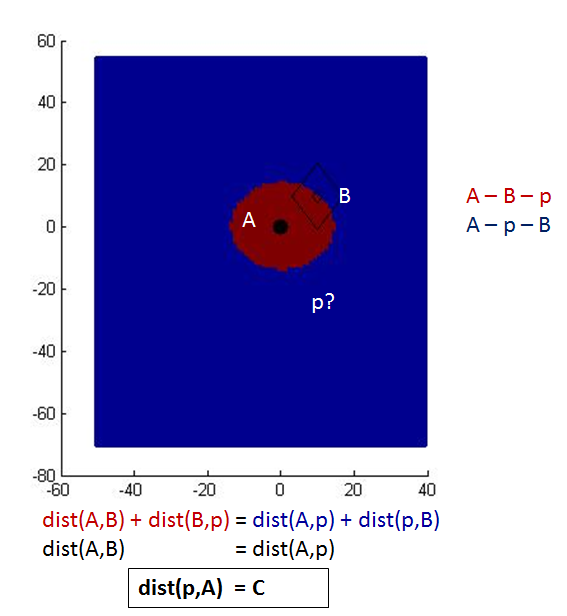
\includegraphics[scale=1.0]{pics/addl/initial-sample-tsp-sbe.eps}
    \caption{Solution border calcuated by SBE for a two-city TSP.  Result is a circle around city B with a constant radius equivalent to the distance from A to B.}
    \label{fig:initial-sample-tsp-sbe-addl}
\end{center}
\end{figure}

\begin{figure}
\fbox{\begin{minipage}{1.0\textwidth}
Let A-p-B and A-B-p represent the routes specified by two 
solutions.  To find the shape of the border, we set the 
distances of the routes to be equal.
\begin{align*}
dist(p,A) + dist(p,B) &= dist(A,B) + dist(p,B)
\\ dist(p,A) &= dist(A,B)
\\ \sqrt{(p_x-A_x)^2+(p_y-A_y)^2} &= dist(A,B)
\\ (p_x-A_x)^2+(p_y-A_y)^2 &= dist(A,B)^2
\end{align*}
\end{minipage}}

\caption{The border between solutions A-p-B and A-B-p simplifies to a circle}
\label{fig:sbe-simple-eq} 
\end{figure}



\begin{figure}
\fbox{\begin{minipage}{1.0\textwidth}
Let A-B-C-p-D and  A-p-B-C-D represent the routes specified by two 
solutions.  To find the shape of the border, we set the 
distances of the routes to be equal.
\begin{equation*}
\begin{split}
dist(A,B) + dist(B,C) + dist(p,C) + dist(p,D) =\\
dist(p,A) + dist(p,B) + dist(B,C) + dist(C,D)\\\\
dist(p,A) - dist(p,B) + dist(p,C) - dist(p,D) =\\
dist(B,C) + dist(C,D) - dist(A,B)
\end{split}
\end{equation*}
\end{minipage}}%end fbox
\caption{The border between solutions A-B-C-p-D and A-p-B-C-D has a non-trivial simplification}
\label{fig:sbe-complex-eq} 
\end{figure}

\begin{figure}
\begin{center}
\includegraphics[scale=0.25]{pics/FiveCityFourFixed_0-3.dat.eps}
\caption{Various ideal PS Maps demonstrating a pattern of correlation between fixed city location and solution borders.}
\label{fig:five_city_tsps_scbias_motivation}
\end{center}
\end{figure}



\begin{algorithm}
\caption{Sampling-Classification+Bias}   
\label{alg:sc+bias}
\small
\begin{algorithmic}[1] %interval between lines labeled with line numbers
  
  \State Let $alpha \in (0.0,1.0)$
  \State Let $sampleRate \in (0.0,1.0)$
  \State Let $problemSpace \leftarrow$ set of problem instances
  \State Let $pollingRadius \in \mathbb{Z}^+$ 
  \State Let $biasFactor \in \mathbb{Z}^+$ 
  \State Let $cityRadius \in \mathbb{Z}^+$ 
  \State $totalNumSamples \leftarrow |problemSpace| * sampleRate$
  \State $numNearSamples \leftarrow \frac{biasFactor * totalNumSamples}{1+biasFactor}$
  \For{$1 \dots numNearSamples$}
    \State Randomly select unsolved problem instance within $cityRadius$ of city
    \State Generate solution for unsolved problem instance
    \State Add problem instance \& solution to PS Map
  \EndFor

  \For{$numNearSamples+1 \dots totalNumSamples$}
    \State Randomly select unsolved problem instance outside of $cityRadius$ of city
    \State Generate solution for unsolved problem instance
    \State Add problem instance \& solution to PS Map
  \EndFor

  \ForAll{$u \in$ unsolved problem instances}
    \State Let $rad \leftarrow pollingRadius$
    \While{$u$ is unsolved \& $rad < radiusOf(problemSpace)$}
      \State Score solutions of problem instances within $rad$ of $u$
      \If{there exists a unique solution with the maximum score}
        \State Assign solution to $u$
      \Else 
        \State $rad \leftarrow rad * 2$
      \EndIf
    \EndWhile
    \If{there does not exist a unique solution with the maximum score}
      \State Randomly choose one of the top solutions
    \EndIf
    \State Add problem instance \& solution to set of pending entries 
  \EndFor
  \State Add pending entries to PS Map 
\end{algorithmic}
\end{algorithm}






\begin{algorithm}
  \caption{Sampling-Classification + Active Learning}   
  \label{alg:sc+al}
  \small
  \begin{algorithmic}[1] % enter the algorithmic environment, specifying lines per line number marking
    \State Let $alpha \in (0.0,1.0)$
    \State Let $sampleRate \in (0.0,1.0)$
    \State Let $problemSpace \leftarrow$ set of problem instances
    \State Let $pollingRadius \in \mathbb{Z}^+$ 
    \State Let $landslide \in  \mathbb{Z}^+$ 
    \State $totalNumSamples \leftarrow |problemSpace| * sampleRate$
    \State $numInitialSamples \leftarrow totalNumSamples * alpha$ 
    \State $usedSamples  \leftarrow numInitialSamples$
    \For{$1 \dots numInitialSamples$}
      \State Randomly select unsolved problem instance
      \State Generate solution for unsolved problem instance
      \State Add problem instance \& solution to PS Map
    \EndFor
  
     \ForAll{$u \in$ unsolved problem instances}
       \State Let $V \leftarrow$ solutions of problem instances within $pollingRadius$ of $u$ ordered by decreasing count
       \If{$|V| = 1$} \hspace{60pt} //there is only one solution
         \State Assign solution to $u$
       \ElsIf {$\frac{count(V_0)}{count(V_1)} \geq landslide$} \hspace{35pt} //highest score divided by second-highest
          \State Assign $V_0$ to $u$
        \ElsIf {$usedSamples < totalNumSamples$}
          \State Solve $u$ and assign solution
        \Else
          \State {Expand radius and assign solution as with Sampling-Classification}
        \EndIf
      \EndFor

  \end{algorithmic}
\end{algorithm}


\section{Sampling-Classification with Bias (SC+bias)}

The \textit{sampling-classification with bias} (SC+bias) technique, described in Algorithm \ref{alg:sc+bias}, attempts to exploit the observation that certain constraints -- for example, known city locations -- indicate boundaries between solutions.  This relationship is suggested by Figures \ref{fig:ideal-ps-map-addl} and \ref{fig:five_city_tsps_scbias_motivation}, and the proof in Figure \ref{fig:dtsp-city-proof} demonstrates that static city locations \textit{must} lie on a border between two solutions.  Thus in SC+bias, the problem instance  samples are biased towards the known city locations in the hope that additional samples in these regions will allow the classification step to discover the borders between solutions with greater accuracy. After gathering the additional samples, this technique assigns solutions to unsolved instances in the same manner as the SC technique.

This technique relies on two additional parameters.  The \textit{city radius} parameter is a radius defining a pool of problem instances that are ``near'' a city location; instances outside this radius are considered not to be near the city.  The \textit{bias factor} parameter defines the ratio of the number of near city points to the number of non-near city points selected in the initial random sample.  For example, a bias factor of three indicates that three times as many near-city points as non-near points will be selected.

The use of this technique is specific to TSP problems.  Although there is consideration for taking into account specific constraints of static problem characteristics to inform sampling bias, it is not clear how this applies in a general case.  Thus, this technique was tested only on the TSP domain.

\begin{algorithm}
\caption{Solution Border Estimation - trace}   
\label{alg:sbe}
\small
\begin{algorithmic}[1] 
  \State Let $sampleRate \in (0.0,1.0)$
  \State Let $problemSpace \leftarrow$ set of problem instances
  \State $totalNumSamples \leftarrow |problemSpace| * sampleRate$

  \For{$1 \dots totalNumSamples$} \label{alg:sbe:initsample}
    \State Randomly select unsolved problem instance
    \State Generate solution for unsolved problem instance
    \State Add problem instance \& solution to PS Map
  \EndFor

  \State $borderSet \leftarrow \emptyset$
  \For{each pair of problem instances $p,q$ with differing solutions $s_p,s_q$} \label{alg:sbe:binarysearch}
    \State use binary search to find pair of adjacent problem instances with differing solutions \label{alg:sbe:dobinarysearch}
    \State $border \leftarrow$ DoTrace($p,s_p,s_q,\emptyset$)
    \State Add $border$ to $borderSet$
  \EndFor

  \State find intersections of borders to determine regions \label{alg:sbe:findintersections}

  \ForAll {region r} \label{alg:sbe:regions}
    \State find problem instance to serve as regional representative
    \State find best solution for this problem instance
    \State assign solution to all problem instances in the region
  \EndFor

  \Function{DoTrace}{$instance$,$solution$,$altSolution$,$border$}
    \State add $instance$ to $border$
    \ForAll {problem instance $p_a$ adjacent to $instance$}
      \If {$p_a$ is adjacent to a problem instance with where $altSolution$ is better than $solution$}
        \State add $p_a$ to $border$
        \State DoTrace($p_a$,$solution$,$altSolution$,$border$)
      \EndIf
    \EndFor
    \State \Return $border$
  \EndFunction
      

\end{algorithmic}
\end{algorithm}


\section{Sampling-Classification with Active Learning (SC+AL)}
The \textit {sampling-classification with active learning} (SC+AL) algorithm modifies the SC (sampling and classification) technique to utilize active sampling rather than random sampling to select problem instances to solve (Algorithm \ref{alg:sc+al}).  This algorithm adds two paramters, \textit{alpha} and \textit{landslide}.  The alpha parameter represents the fraction of the total number of problem instances that will be selected through random sampling.   The landslide threshold is used to determine whether the voting by the nearest neighbors is ambiguous.  For example, a sample rate of .01 in a problem space with 10,000 instances results in a total of 100 samples.  Assuming an alpha of 0.2, an initial random sampling of 20 problem instances will be solved.  The remaining 80 samples will be  chosen after evaluating the fixed-radius neighbors of unsolved problem instances. If the fixed-radius neighbors of an unsolved problem instance indicate little or no ambiguity when approximating its solution, then the problem instance is assigned a solution as in SC, by a plurality vote.  However, if the fixed-radius neighbors do indicate ambiguity, then the problem instance is solved heuristically if the total allocation of problem instance samples has not been exhausted.  In this algorithm, ambiguity refers to either zero fixed-radius neighbors, or more than one fixed-radius neighbor in which the number of occurrences of the best solution divided by the number of occurrences of the second-best solution does not meet the \textit{landslide} threshold.  Figure \ref{fig:initial-sample-tsp-activelearning-addl} provides a pictorial representation of ambiguous problem instances requiring evaluation by the solver, and landslide and unanimous problem instances which can be classified with nearest neighbor.

\begin{figure}
\begin{center}
    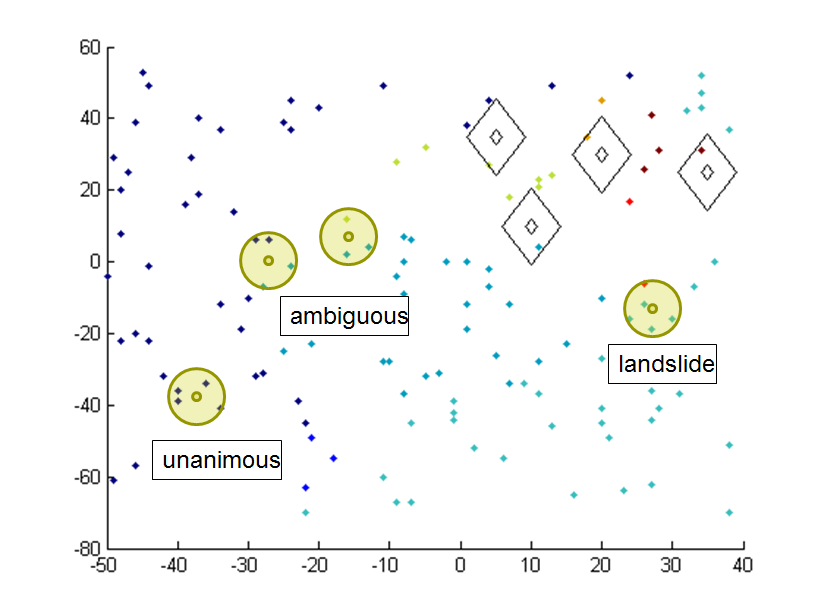
\includegraphics[scale=0.7]{pics/addl/initial-sample-tsp-activelearning.eps}
    \caption{Initial sampling of a problem space augmented with type of resolution for several unsolved problem instances}
    \label{fig:initial-sample-tsp-activelearning-addl}
\end{center}
\end{figure}

\section{Solution Border Estimation (SBE)}

This next technique differs from previous algorithms in that instead of using a nearest neighbor approach to classify unsolved problem instances to known solutions, this technique uses the problem domain's objective function to find the borders between solutions, thus allowing it to classify all the problem instances within a region.  The intent is that this technique will be more accurate than the previous algorithms, but does require the availability of an objective function and can be more computationally expensive.

The \textit{solution border estimation} (SBE) technique calculates solutions to a random sample of the problem instances as in the previous algorithms.  Then, for every pair of solutions, SBE calculates a border in the problem space where one solution becomes better than the other.  The combination of these borders creates a set of regions within the problem space.  Because the borders that create the regions are determined only by a pair of solutions, there is no guarantee that some third solution is not preferable within any region.  To resolve this uncertainty, the algorithm determines the best solution within a region by solving one problem instance within each region, and assigning that solution to all problem instances in the region.  

Ideally, these borders would be calculated by equating the objective functions representing each solution and finding a closed-form expression for the boundary location, such as shown in Figures \ref{fig:initial-sample-tsp-sbe-addl} and \ref{fig:sbe-simple-eq} for a 2-city TSP problem. However, this approach is not practical for large problems or problems that are not easily expressed with an objective function.  As an example of the difficulty presented by a larger problem, consider resolving the border between 5-city TSP solutions A-B-C-p-D and A-p-B-C-D, where p is the unknown location and A, B, C, and D represent known locations.  This results in a non-trivial equation in Figure \ref{fig:sbe-complex-eq} with four radicals (pairwise distances) and a constant.  Therefore, my implementation, \textit{SBE-trace}, uses an approximation of the SBE technique, as described in Algorithm \ref{alg:sbe}.    

  Figure \ref{fig:sbe-steps} illustrates the SBE-trace algorithm.  First, two solved problem instances with differing solutions are selected (a).  Next, a binary search is applied to the space between the two solved instances to find two adjacent problem instances that have different solutions (b).  Then, the remainder of the border is discovered by testing neighboring points for adjacency to a problem instance with the alternate solution, forming a continuous border between the solution regions (c,d).  Applying this procedure in a pairwise fashion to the remaining discovered solutions (e,f) creates an approximation of the skeletal PS Map (g).  Finally, sampling within each region yields an approximate PS Map (h).




\begin{figure}
\begin{center}
    \includegraphics[scale=.9]{pics/sbe-steps.eps}
    \caption{Skeletal PS Map created by SBE-trace procedure}
    \label{fig:sbe-steps}
\end{center}
\end{figure}





\section{Support Vector Machine (SVM)}
The \textit{support vector machine} approach, described in Algorithm \ref{alg:svm}, utilizes a support vector machine \citep{vapnik95svm} to classify unsolved problem instances into classes consisting of known solutions.  A support vector machine classifies inputs into one of two classes by calculating a hyperplane that splits the input space into two regions, one for each class, that  lies as far as possible from any input instance.  A simple example of this is shown in Figure \ref{fig:initial-sample-svm-addl}.  An advantage of this classifier is that it scales to high-dimensional spaces.  SVMs employ a ``kernel trick'' that allows them to calculate a hyperplane when the inputs are not linearly separable, as is typically the case  in the plan spaces that I have studied.

In this algorithm, an initial sample of problem instances are solved to generate solutions, as in the SC technique.  I train the SVM with the problem instances' variable characteristics and the high-quality solution generated by the heuristic solver.    After training, the unsolved instances are assigned solutions based on  the SVM's classifications.

\begin{figure}
\begin{center}
    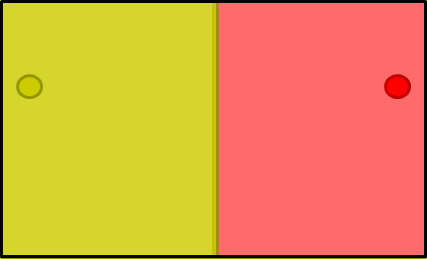
\includegraphics[scale=1.0]{pics/addl/initial-sample-svm.eps}
    \caption{Expected classification of unsolved problem instances by SVM algorithm given two solved problem instances from the initial sample.}
    \label{fig:initial-sample-svm-addl}
\end{center}
\end{figure}


\begin{algorithm}
\caption{Support Vector Machine}   
\label{alg:svm}
\small
\begin{algorithmic}[1] % enter the algorithmic environment, specifying lines per line number marking
  
  \State Let $sampleRate \in (0.0,1.0)$
  \State Let $problemSpace \leftarrow$ set of problem instances
  \State $totalNumSamples \leftarrow |problemSpace| * sampleRate$
  \For{$1 \dots totalNumSamples$}
    \State Randomly select unsolved problem instance
    \State Generate solution for unsolved problem instance
    \State Add problem instance \& solution to PS Map
    \State Add problem instance features \& solution to SVM training set
  \EndFor
  \State Train SVM
  \ForAll{unsolved problem instances}
    \State Add problem instance and SVM classification to PS Map
  \EndFor
\end{algorithmic}
\end{algorithm}

\begin{algorithm}
\caption{Support Vector Machine + Solution Border Estimation}   
\label{alg:svm+sbe}
\small
\begin{algorithmic}[1] % enter the algorithmic environment, specifying lines per line number marking
  
  \State Let $alpha \in (0.0,1.0)$
  \State Let $sampleRate \in (0.0,1.0)$
  \State Let $problemSpace \leftarrow$ set of problem instances
  \State $totalNumSamples \leftarrow |problemSpace| * sampleRate$
  \State $numInitialSamples \leftarrow totalNumSamples * alpha$ 
  \For{$1 \dots numInitialSamples$}
    \State Randomly select unsolved problem instance
    \State Generate solution for unsolved problem instance
    \State Add problem instance \& solution to PS Map
    \State Add problem instance features \& solution to SVM training set
  \EndFor

  \For{each pair of problem instances with differing solutions $s_p,s_q$} \label{alg:svmsbe:binarysearch}
    \State use binary search to find pair of adjacent problem instances with differing solutions
    \State Add pair of problem instances and their solutions to SVM training set
  \EndFor

  \State Train SVM
  \ForAll{unsolved problem instances} \label{alg:svmsbe:makemap}
    \State Add problem instance and SVM classification to PS Map
  \EndFor
\end{algorithmic}
\end{algorithm}



\begin{algorithm}
\caption{Select from Sampled Solutions}   
\label{alg:sss}
\small
\begin{algorithmic}[1] 
  
  \State Let $sampleRate \in (0.0,1.0)$
  \State Let $problemSpace \leftarrow$ set of problem instances
  \State Let $pollingRadius \in \mathbb{Z}^+$ 
  \State $totalNumSamples \leftarrow |problemSpace| * sampleRate$
  \For{$1 \dots totalNumSamples$}
    \State Randomly select unsolved problem instance
    \State Generate solution for unsolved problem instance
    \State Add problem instance \& solution to PS Map
  \EndFor

  \ForAll{$u \in$ unsolved problem instances}
    \State{Generate utility of $u$ for each known solution in PS Map}
    \If{there does not exist a unique solution with the maximum score}
      \State Randomly choose one of the top solutions
    \EndIf
    \State Add problem instance \& solution to set of pending entries 
  \EndFor
  \State Add pending entries to PS Map 
\end{algorithmic}
\end{algorithm}


\section{Support Vector Machine with Solution Border Estimation (SVM+SBE)}
The \textit{support vector machine with solution border estimation} (SVM+SBE) technique (Algorithm \ref{alg:svm+sbe}) utilizes a fraction of the total allocated samples to create an initial sample of problem instances from which to generate a set of known solutions.  For each combination of pairwise problem instances that have different solutions, the SBE technique is used to find a pair of problem instances that lie on the border between the two solutions.  These border points and their solutions are added to the SVM training set.  Finally, the unsolved problem instances are assigned solutions as dictated by the SVM results.  An illustration of this is presented by Figure \ref{fig:initial-sample-svmsbe-addl}.


\begin{figure}
\begin{center}
    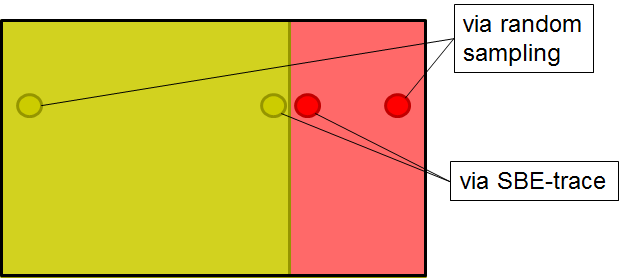
\includegraphics[scale=1.0]{pics/addl/initial-sample-svmsbe.eps}
    \caption{Expected classification of unsolved problem instances by SVM+SBE algorithm given two solved problem instances from the initial sample and two from the SBE augmentation step.}
    \label{fig:initial-sample-svmsbe-addl}
\end{center}
\end{figure}


\section{Select from Sampled Solutions (SSS)}
\label{sec:sss}
The \textit{select from sampled solutions} (SSS) technique calculates solutions to a random sample of the problem instances.  This technique assigns solutions to each unsolved problem instance by computing the utility of each of the discovered solutions when applied to the unsolved instance, and assigning the maximum-utility solution.  In the case of continuous objective functions, which creates large homogeneous solution regions, this process generates a PS Map identical to that of SBE-trace.  However, because it must determine the maximum utility solution for every problem instance in the space, this algorithm risks performance degradation as the problem size increases.  For example, for a map representing a DTSP with two variable cities consisting of $\textrm{12,000}^{\textrm{2}}$ problem instances, SSS would entail evaluating every unknown solution for every problem instance.  However, in situations in which the number of stored solutions is small or the cost of calculating the utility is cheap enough, the discovered solutions could be stored, rather than a complete map.  This could mitigate the disadvantage that SSS may encounter relative to SBE-trace.

One interesting feature of this algorithm is that it can be used to remove errors in ideal maps caused by the use of heuristics when solving problem instances.  Heuristic solvers may assign different solutions to differing problem instances that in fact do have identical solutions. The  application of this algorithm can mitigate this type of error by considering all the discovered solutions within the problem space.  Visually, this has the effect of ``smoothing'' the solution regions into more regular shapes within the TSP and knapsack problem domains.

\section{Algorithm Analysis}
\label{sec:complexity}
I have analyzed these algorithms primarily in terms of the number of problem instances that must be resolved by the heuristic solver.  Solving a problem instance with the heuristic solver takes the highest amount of time for a single problem instance; however, many of the solutions involve less expensive operations over a large number of problem instances and thus the heuristic solve time cannot be assumed to dominate the complexity expresssion.  

Let $H$ represent the time complexity required to solve a single problem instance with a heuristic solver, and let $s$ represent the sample rate.  $P$ will represent the size of the problem space and $K$ will represent the complexity of the fixed-radius neighbor search.  A brute-force fixed-radius neighbor search is $O(n)$ in the number of candidate neighbors.  However, other approaches can be appropriate depending on the number of candidate neighbors, which varies as function of the sample size.  To accommodate this variability, the final complexities listed in Table \ref{tab:summary-of-complexity} present the complexities using a generic $K$ for the fixed-radius neighbor search as well as assuming a worst-case complexity of  $O(n)$.

\subsubsection{SC Algorithm} The Sampling-Classification (SC) uses an initial sample of solved problem instances to perform nearest neighbor-like classification of the unsolved problem instances.  For the SC algorithm, the initial loop samples the complete problem space and solves an initial sample of problem instances.  This complexity is $O(HsP)$.  Next, the remaining $(1-s)P$ problem instances must be solved.  For each instance, the algorithm runs the fixed-radius neighbor search repeatedly until either there is a plurality of solutions within SC's expanding radius, or the radius encompasses the complete problem space.  Since the radius doubles with each iteration, the maximum number of iterations possible per problem instance is $log_2P$.  Thus the complexity for SC is $O(HsP + (1-s)PKlogP)$, where $K$ is the complexity of fixed-radius neighbor search.  The intent of these algorithms is for $s$ to be small, particularly when $H$ is large.  Therefore, it is not clear whether the first term, which is a product of a large and small number, dominates or is dominated by the second term, which is a product of a number near one, the size of the problem space, its log, and the complexity of the fixed-radius neighbor search.

\subsubsection{SC+Bias Algorithm} The SC+Bias algorithm is identical to SC except that the initial  sampling is biased towards sampling specific locations in the problem space. There is some expense to identify the set of problem instances that are within the radius of a city, but this one-time cost, amortized over repeated runs, is negligible.  Thus the calculations are the same as the SC algorithm, resulting in the complexity of $O(HsP + (1-s)PKlogP)$.

\subsubsection{SC+AL Algorithm} SC with Active Learning (SC+AL) splits the total allocation of samples between the initial random and targeted sampling during the classification stage. The complexity of the SC+AL algorithm must consider the alpha parameter that determines the initial fraction of problem instances  to be solved heuristically through random sampling.  The complexity of this step is $O(Hsp\alpha)$.  The remaining problem instances to be solved heuristically are determined by the  utility of the solutions discovered when polling within the radius of the problem instance.  The complexity of this step is $O(Hsp(1-\alpha))$.  Combining these two terms,  $HsP\alpha$ + $HsP(1-\alpha)$, simplifies to the same initial term as the previous algorithms, $HsP$.  The cost of solving the remaining $(1-s)P$ problem instances is, in the worst case, the cost of expanding the polling radius as in SC.  This results in a total complexity of $O(HsP + (1-s)PKlogP)$, again the same as the SC algorithm.

\subsubsection{SBE-trace Algorithm} Support Border Estimation-trace (SBE-trace) is an approximation of SBE, which calculates borders between known solutions using the domain's objective function. The SBE-trace algorithm is limited to two dimensions, which is used to simplify its complexity analysis.  As with the previous algorithms, the initial sampling  is again of complexity $O(HsP)$.  The loop starting at line \ref{alg:sbe:binarysearch} runs for each pairwise combination of solutions for a total of $n(n-1)$ iterations, where $n$ is the number of solutions.  The number of solutions is the result of solving the initial sample of problem instances. Thus, $n$ is equal to $sP$ and the loop executes $sP(sP-1)$ times.

Each loop iteration executes a binary search that may in the worst case span the problem space and therefore has a complexity of $logP$.  Each iteration also executes the \textsc{DoTrace} function, which executes a loop that considers the seven adjacent problem instances to a given instance.  The recursion then continues the evaluation for the length a complete border, which is at worst the size of the problem space.  Thus, the complexity of the function is $7P$.  As mentioned above, these two operations execute $sP(sP-1)$ times, for a total complexity of $sP(sP-1)(logP + 7P)$, simplifying to $O(s^2P^3)$.

The process at line \ref{alg:sbe:findintersections} of finding the points at the intersections of borders requires looping through each pairwise set of borders to find points that exist in both borders.  This requires $B(B-1)$ loop iterations, where $B$ is the number of borders, for a complexity of $O(B^2)$.  Recalling that the number of borders is $O((sP)^2)$ and that a border may at most contain $P$ points, the overall complexity of this operation is $O(((sP)^2)^2 \times P)$, which simplifies to $O(s^4P^5)$.

The final loop at line \ref{alg:sbe:regions} requires selecting a solution for  one problem instance in each region resulting in a complexity of $O(sPR)$, where $sP$ is the number of solutions to evaluate, and $R$ is the number of regions generated by the border intersections.  In two-dimensional spaces, the number of regions generated by dividing a space with $n$ lines or circles is $O(n^2)$.  Intuitively, this can be demonstrated by observing that the $i^{th}$ line that divides a space adds at most $i$ regions to the space, thereby creating $\sum\nolimits_{i=1}^{n}i = \frac{n(n-1)}{2}$ regions for a complexity of $O(n^2)$.  Replacing $n$ with the number of borders, $O((sP)^2)$, and substituting for $R$, the complexity of this loop is $O(sP \times s^4P^4) = O(s^5P^5)$.

The sum of all of these terms is $O(HsP + s^2P^3 + s^4P^5 + s^5P^5)$.  The fourth term dominates the second and third terms, simplifying to  $O(HsP + s^5P^5)$.  As before, it is not clear which, if either, of the terms dominates the expression, and thus both of them are preserved.

\subsubsection{SVM Algorithm} The SVM algorithm trains a support vector machine with the initial random sample in order to classify unsolved problem instances to one of the discovered solutions.  The SVM and SVM+SBE algorithms rely heavily on support machine training algorithms, which has a generally accepted upper bound of $O(n^3)$ in the number of training instances \citep{bottou2007support,List09svm-optimization}.  The complexity of the SVM algorithm is readily calculated as the sum of the complexity of sampling, training, and possibly classification: $O(HsP + (1-s)^3P^3 + (1-s)P)$.  Dropping the final term because of the domination of the middle term results in an SVM algorithm complexity of $O(HsP + (1-s)^3P^3)$

\subsubsection{SVM+SBE Algorithm} SVM+SBE splits its total sample allocation between the initial random sample and targeted sampling within the regions between problem instances with differing solutions.  The SVM+SBE algorithm complexity is similar to the SVM complexity, but uses an alpha parameter that determines the fraction of sampled instances that will be derived from solution border estimation.  Because of this, the complexity of the initial sample is $O(HsP\alpha)$.  The loop starting at line \ref{alg:svmsbe:binarysearch} runs a maximum of $(1-\alpha)sP$ times and has the same binary search as line \ref{alg:sbe:dobinarysearch} of the SBE - trace algorithm.  Each of the border problem instances is solved with an $O(H)$-complexity heuristic search.  Thus the complexity of this loop is $O((1-\alpha)P(H+logP))$.  The SVM training is again $O(n^3)$ in the number of training instances for a complexity of $O(s^3P^3)$.  The last loop at line \ref{alg:svmsbe:makemap} iterates over the $(1-s)P$ unsolved problem instances and places them in the PS Map.  Summing the terms results in a complexity of $O(HsP\alpha + (1-\alpha)sP(H+logP) + s^3P^3 + (1-s)P)$, which simplifies to  $O(HsP + s^3P^3)$.

\subsubsection{SSS Algorithm} Select from sampled solutions (SSS) tests each solution discovered during the initial sample against each of the unsolved problem instances.  The SSS algorithm requires $O(HsP)$ for the initial sample and for each of  the remaining $(1-s)P$ unsolved instances, it must evaluate each of the discovered solutions.  Assuming each sample results in a unique solution, this results in the worst case, $(1-s)P \times sP$ evaluations, or $O(sP^2)$ assuming a small $s$.  Thus, the complexity of SSS is $O(HsP + sP^2)$.

\begin{table}
\begin{center}
  \begin{tabular}{|p{2cm}|p{5cm}|p{5cm}|}
    \hline
    \textbf{Algorithm} & \textbf{Complexity} & \textbf{K = O((1-s)P)}     \\ \hline
    \textbf{SC} &       $O(HsP + (1-s)PKlogP)$   & $O(HsP + (1-s)^2P^2logP)$ \\ \hline
    \textbf{SC+bias} &  $O(HsP + (1-s)PKlogP)$   & $O(HsP + (1-s)^2P^2logP)$ \\ \hline
    \textbf{SC+AL} &    $O(HsP + (1-s)PKlogP)$   & $O(HsP + (1-s)^2P^2logP)$ \\ \hline
    \textbf{SBE} &      $O(HsP + s^5P^5)$         &\\ \hline
    \textbf{SSS} &      $O(HsP + sP^2)$           &\\ \hline
    \textbf{SVM} &      $O(HsP + (1-s)^3P^3)$     &\\ \hline
    \textbf{SVM+SBE} &  $O(HsP + s^3P^3)$         &\\ \hline
  \end{tabular}
  \caption{Summary of PS Map approximation complexity. H is the complexity of generating a high-quality solution, s is the sample rate, P is the number of instances in the problem space, and K is the complexity of the fixed-radius neighbor search.}
  \label{tab:summary-of-complexity}
\end{center}
\end{table}
